\documentclass[twocolumn,10pt]{article}

\usepackage{authblk}
\usepackage{bera}
\usepackage[utf8]{inputenc}
\usepackage[T1]{fontenc}
\usepackage{graphicx}
\usepackage{booktabs}
\usepackage{url}
\usepackage[font=small,skip=3pt]{caption}
\usepackage[nolist]{acronym}
\usepackage[compact]{titlesec}
\titlespacing*{\section}{0pt}{5pt}{2pt}
\titlespacing*{\subsection}{0pt}{3pt}{1pt}
\setlength{\textfloatsep}{6pt}
\setlength{\floatsep}{5pt}

\usepackage[a4paper,
    top=1.5cm,
    bottom=1.5cm,
    left=1.8cm,
    right=1.8cm
]{geometry}

\begin{acronym}
\acro{TF-IDF}{term frequency--inverse document frequency}
\acro{SVM}{linear support vector machine}
\acro{LR}{logistic regression}
\acro{MNB}{Multinomial Naive Bayes}
\acro{EDA}{easy data augmentation}
\acro{KW}{keyword}
\end{acronym}

% TITLE
\title{Clinical Text or Corpus Structure? Medical Specialty Classification with Sparse Models and Clinical BERT}

% AUTHORS
\author{Group XXX, Author 1 (xx\%), Author 2 (xx\%), Author 3 (xx\%) and Author 4 (xx\%)}
\date{}

\begin{document}

\maketitle

\raggedbottom

\section{Introduction}

\noindent
Classifying clinical records into medical specialties is challenging due to heterogeneous documentation and overlap between clinical domains. Clinical narratives often contain information relevant to multiple specialties, making their automatic categorisation ambiguous. This project explores natural language processing approaches to specialty classification on 12 specialties and addresses the following research question: \textit{How effectively can natural language processing models classify clinical records into medical specialties using clinical text alone, and how much of the attainable performance comes instead from structural properties of the corpus?}
To answer it, we compare a sparse \ac{SVM}, a sparse \ac{LR} with data augmentation, and a fine-tuned clinical Transformer, and we report the contribution of the clinical text and of two corpus properties separately.

\section{Data}

\subsection{Data Analysis}

\noindent The training dataset comprises 2,669 clinical records across 12 medical specialties. Each record contains a specialty label and four input fields: description, sample name, transcription, and keywords. The class distribution is highly imbalanced: Surgery accounts for 893 records (33.5\%), whereas Dermatology contains only 25 (0.9\%) (Figure~\ref{fig:dist}, Appendix~A). This imbalance motivates the use of per-class metrics alongside overall performance measures.

\noindent The source CSV contained seven records with missing fields, six lines with additional empty fields, and three transcriptions split across consecutive lines. We filled missing fields with empty strings, removed empty trailing fields, and rejoined the fragmented transcriptions; no record was discarded. The resulting dataset contains one empty description, seven empty sample names, 31 empty transcriptions, and 450 records without keywords. Transcriptions have a median of 386 words. We highlight three observations.

\noindent\textbf{O1: the first keyword is the label.} In all 2,219 records with non-empty keywords, the first keyword names the assigned specialty (``cardiovascular / pulmonary, chest pain, \dots''). Missing keywords are not random: 27 of the 41 Psychiatry-Psychology and 90 of the 212 General Medicine records have none, against 63 of the 893 Surgery records. In the test file, 320 of the 398 records also start with a specialty name.

\noindent\textbf{O2: the same note is listed under several specialties.} 1,528 records (57.2\%) share an identical non-empty transcription with at least one record assigned to a different specialty. For example, two records describing the same lower-extremity venous Doppler examination have identical input fields but are labelled Cardiovascular-Pulmonary and Radiology. The data derive from the MTSamples collection \cite{mtsamples}, which lists a note once under each relevant specialty. Of the 731 transcriptions that occur more than once, 730 carry a different label on every copy, mostly a pair ``organ specialty + Surgery'' or ``organ specialty + Radiology''. A model that sees only the text therefore cannot exceed 70.1\% accuracy (predicting the most frequent label of each distinct transcription).

\noindent\textbf{O3: the test set shares notes with the training set.} 239 of the 398 test transcriptions occur in the training set. Given O2, a model that memorises the label of a training note is systematically wrong on its test copy.

\subsection{Data Augmentation}

\noindent Augmentation is applied to the minority classes (fewer than 100 training records: Dermatology, Psychiatry-Psychology, Ophthalmology and Neurosurgery), which receive three augmented copies of each record (2,135 $\rightarrow$ 2,657 training records). We compare two strategies from \ac{EDA} \cite{wei2019eda}: \textbf{random swap}, which exchanges three random pairs of words, and \textbf{swap + deletion}, which deletes each word with probability 0.1 and then swaps 5\% of the word positions. Synonym replacement was not used because general-purpose thesauri do not cover clinical vocabulary. Augmentation is applied \emph{only to the training split}: a first version that augmented before splitting placed near-identical copies of the same note in both splits and inflated accuracy from 77.3\% to 84.1\% (minimum per-class F1 from 0.33 to 0.69). Each augmented configuration is run with three augmentation seeds.

\section{Models}

\noindent All text models read the four fields concatenated, \emph{with the first keyword removed} (O1), so that they learn from clinical content. Two inference rules, derived from O1--O3 and independent of the text model, are layered on top:
\textbf{(R1) Keyword rule:} if the first keyword names a specialty, it is returned.
\textbf{(R2) Duplicate-note rule:} if the transcription of a record occurs in the training data, the labels of its training copies are excluded and the highest-scoring remaining label is returned. R2 uses training data only.

\noindent\textbf{Baseline.} \ac{MNB} on \ac{TF-IDF} features of the description, lower-cased and Snowball-stemmed (the course baseline).

\noindent\textbf{Model 1: \ac{TF-IDF} + \ac{SVM}.} Lower-cased word unigrams, sublinear term frequency ($1+\log \mathrm{tf}$) and a minimum document frequency of 2. Stop words are kept, since \ac{TF-IDF} already assigns them low weights. A \ac{SVM} with balanced class weights (each class weighted inversely to its frequency) addresses the imbalance.

\noindent\textbf{Model 2: n-grams + \ac{LR} + augmentation.} Word uni- and bigrams (to capture terms such as ``blood pressure'' or ``no fracture''), a class-balanced \ac{LR}, and the augmentation of Section~2.2. We also evaluate the group's initial choice of collapsing repeated transcriptions into one record labelled with the most frequent specialty (mode de-duplication).

\noindent\textbf{Model 3: fine-tuned Clinical BERT.} Bio\_ClinicalBERT \cite{alsentzer2019}, a BERT model \cite{devlin2019} pre-trained on biomedical literature and on clinical notes from MIMIC-III \cite{johnson2016mimic}, with a linear classification layer on the \texttt{[CLS]} representation; all weights are fine-tuned. No lower-casing, stemming or stop-word removal is applied, as the model uses its own WordPiece tokenizer and was pre-trained on raw text. Records have a median of 746 tokens and 72\% exceed BERT's limit of 512 tokens, so the input is ordered \emph{sample name [SEP] description [SEP] keywords [SEP] transcription}: truncation then removes only the end of the transcription. Class imbalance is handled with a class-weighted cross-entropy loss.

\noindent The submitted system is Model 3 with R1 and R2: on the official test set, R1 labels 320 records and Clinical BERT the remaining 78, of which 30 are constrained by R2.

\section{Experimental Setup}

\noindent The official test set was used only to produce \texttt{results.txt}. All results come from our own test set: a stratified 80/20 split of the training data (2,135 / 534 records, \texttt{random\_state}=42), identical for all models. The split is random rather than grouped by transcription, so that, as in the official test set (O3), 240 of the 534 test records have a copy in the training split. Metrics are accuracy, macro-F1 and the minimum per-class F1. Each model is reported (i) alone, (ii) with R2, (iii) with R1 and R2 (\emph{full}), and (iv) on the 94 test records without keywords, which are the only records decided by the text model in the full system (\emph{no-KW}).

\subsection{Parameters/Hyperparameters}

\noindent\textbf{Model 1:} regularisation constant $C=0.3$ (inverse strength of the penalty on large weights). \textbf{Model 2:} $C=10$, L2 penalty, 3,000 iterations. \textbf{Model 3:} 4 epochs, AdamW \cite{loshchilov2019} with learning rate $2\cdot10^{-5}$ and weight decay 0.01, linear warm-up over the first 10\% of steps followed by linear decay, batch size 8 with 2 gradient-accumulation steps (effective batch 16), gradient clipping at norm 1.0, bf16 mixed precision, maximum length 512 tokens. Model 3 is trained with seeds 42, 7 and 123; seed 42 produces \texttt{results.txt}. Software: scikit-learn 1.7.2 \cite{pedregosa2011}, PyTorch 2.9.1 and Hugging Face Transformers 5.19.0 \cite{wolf2020}; one epoch takes about 16\,s on an NVIDIA RTX 5080.

\section{Results}

\begin{table}[t]
\centering
\footnotesize\setlength{\tabcolsep}{2.1pt}
\begin{tabular}{lcccccc}
\toprule
 & alone & +R2 & \multicolumn{3}{c}{full (R1+R2)} & no-KW \\
Model & acc & acc & acc & mF1 & minF1 & acc \\
\midrule
Baseline (MNB) & 39.3 & 54.5 & 88.2 & 84.5 & 22.2 & 33.0 \\
M1 TF-IDF + SVM & 44.2 & 76.2 & 94.6 & 93.1 & 79.2 & 69.1 \\
M2 n-grams + LR & 40.1 & 77.3 & 94.8 & 93.3 & 79.6 & 70.2 \\
\quad + random swap & 38.0 & 77.4 & 94.8 & 93.3 & 79.6 & 70.2 \\
\quad + swap + deletion & 37.7 & 77.3 & 94.8 & 93.4 & 79.4 & 70.2 \\
\quad + mode de-dup. & 38.6 & 76.6 & 94.8 & 93.3 & 80.4 & 70.2 \\
M3 Clinical BERT & 54.9 & 75.5 & 95.1 & 92.7 & 80.0 & 72.3 \\
\quad mean of 3 seeds & 55.2 & 76.5 & 95.8 & 93.6 & -- & 75.9 \\
\quad $\pm$ std & 0.4 & 0.9 & 0.7 & 1.0 & -- & 3.7 \\
\quad 3-seed ensemble & -- & -- & 95.9 & 94.4 & 85.1 & 76.6 \\
\bottomrule
\end{tabular}
\caption{Results (\%) on our test set (534 records; no-KW: the 94 records without keywords). M3 rows without annotation use seed 42, the submitted model.}
\label{tab:results}
\end{table}

\noindent Table~\ref{tab:results} summarises the experiments. The best system is Model 3 with both rules: 95.1\% accuracy, 92.7\% macro-F1 and a minimum per-class F1 of 80.0\% (seed 42), and $95.8 \pm 0.7\%$ accuracy over three seeds. Table~\ref{tab:perclass} gives its per-class scores. All 26 errors of this system occur on records without keywords: R1 labelled the other 440 test records correctly. Figure~\ref{fig:cm} is the confusion matrix of Clinical BERT with R2 (without R1), which shows the behaviour of the text model on all 534 records.

\begin{table}[t]
\centering\footnotesize\setlength{\tabcolsep}{2.4pt}
\begin{tabular}{lrrrr|lrrrr}
\toprule
Class & P & R & F1 & n & Class & P & R & F1 & n \\
\midrule
Cardio & 98.2 & 87.1 & 92.3 & 62 & Ortho & 98.4 & 100 & 99.2 & 60 \\
Derm & 80.0 & 80.0 & 80.0 & 5 & ObGyn & 96.2 & 92.6 & 94.3 & 27 \\
Gastro & 92.5 & 94.9 & 93.7 & 39 & Ophth & 93.8 & 100 & 96.8 & 15 \\
GenMed & 73.6 & 92.9 & 82.1 & 42 & Psych & 87.5 & 87.5 & 87.5 & 8 \\
Neuro & 94.4 & 91.9 & 93.2 & 37 & Radio & 97.7 & 97.7 & 97.7 & 44 \\
NSurg & 100 & 93.8 & 96.8 & 16 & Surgery & 100 & 97.8 & 98.9 & 179 \\
\bottomrule
\end{tabular}
\caption{Per-class precision, recall and F1 (\%) of the submitted system (Model 3 + R1 + R2, seed 42) on our test set.}
\label{tab:perclass}
\end{table}

\begin{figure}[t]
\centering
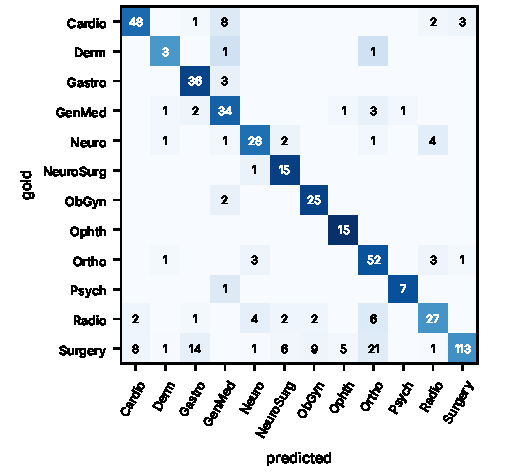
\includegraphics[width=0.92\columnwidth]{figures/confusion_model3.pdf}
\caption{Confusion matrix of Clinical BERT with R2 (without the keyword rule) on our test set: counts, colour normalised per gold class.}
\label{fig:cm}
\end{figure}

\section{Discussion}

\noindent\textbf{Corpus structure dominates.} For Models 1--3, R2 adds 21 to 37 points of accuracy and R1 a further 18 to 20 (Table~\ref{tab:results}). Without R2, the models memorise the label of a training note and are wrong on its test copy (O3); with R2, this becomes an advantage. With both rules, Models 1--3 differ by at most 0.5 points (seed 42), that is, 3 of 534 records.

\noindent\textbf{Where the text model fails.} Figure~\ref{fig:cm} shows that 66 of the 179 Surgery records are predicted as an organ specialty (21 Orthopedic, 14 Gastroenterology, 9 Obstetrics-Gynecology, 8 Cardiovascular-Pulmonary), and that Radiology records are predicted as Orthopedic (6) and Neurology (4). These are the label pairs of O2: the model identifies the organ, whereas the gold label records the type of act (operation or imaging).

\noindent\textbf{Clinical text alone.} The text models are compared on the records they actually decide (no-KW). Clinical BERT reaches $75.9 \pm 3.7\%$ against 69.1\% for the \ac{SVM} and 70.2\% for the \ac{LR}; each of the three seeds exceeds both sparse models, although with 94 records one record is one point. Without the rules, BERT is 10.7 points above the \ac{SVM} (54.9 vs.\ 44.2\%). Pre-training on clinical text therefore helps, but the text models remain about 20 points below the full system.

\noindent\textbf{Augmentation and de-duplication.} Neither augmentation changes the no-KW accuracy (70.2\% in all configurations), and both lower the accuracy without rules (40.1 $\rightarrow$ 38.0 and 37.7\%). The remaining errors stem from records whose correct label is ambiguous, not from a lack of minority-class examples, and the class weights already compensate for the imbalance. Mode de-duplication breaks almost every tie alphabetically: of the repeated transcriptions, none keeps the label Surgery, and the minimum per-class F1 without rules drops from 18.2 to 11.1\%.

\noindent\textbf{Misclassified examples} (submitted system, own test set):
(1) ``Initial clinic visit for foreign body in left eye.'' (sample name ``Gen Med Consult''): gold General Medicine, predicted Ophthalmology. The content is ophthalmic; the gold label reflects the consultation setting, not the organ.
(2) ``Left heart catheterization, coronary angiography, and left ventriculogram. No angiographic evidence of coronary artery disease'': gold Surgery, predicted Cardiovascular-Pulmonary. A cardiology procedure; both labels are defensible, as in O2.
(3) ``Obstructive sleep apnea syndrome. Loud snoring. Schedule an overnight sleep study'' (``Pulmonary Consultation''): gold Cardiovascular-Pulmonary, predicted General Medicine.
(4) ``Preeclampsia, status post delivery with Cesarean section with uncontrolled blood pressure'': gold Obstetrics-Gynecology, predicted General Medicine.
In (3) and (4), and in several emergency-room notes (``Difficulty Breathing -- ER Visit'', gold Cardiovascular-Pulmonary), the note is an outpatient consultation or admission about blood pressure or breathing, a layout that is frequent in General Medicine (212 records, 90 of them without keywords). The model relies on the document type more than on the organ named in the sample name; General Medicine has the lowest precision (73.6\%, Table~\ref{tab:perclass}). (1) and (2) are cases where the gold label is one of several reasonable answers.

\noindent\textbf{Answer to the research question.} Using clinical text alone, the best model (Clinical BERT) classifies 55\% of our test records correctly when notes are shared with the training set, and 76\% of the records without keywords once shared notes are handled. Most of the 95.8\% of the final system comes from two corpus properties (O1 and O2/O3), not from the clinical text. Within the text models, pre-training on clinical notes yields a consistent but modest gain, and augmentation yields none.

\section{Future Work}

\noindent A multi-label formulation (the set of specialties of a note) would model O2 directly and evaluate text models without arbitrary gold labels. For the text model, we would read the 72\% of records longer than 512 tokens in chunks or with a long-context clinical model, train on soft labels reflecting each note's label distribution, and evaluate with grouped cross-validation over more seeds.

\section*{Bibliography}
\noindent\textbf{Use of LLMs.} Claude (Anthropic) was used to analyse the data, write and debug the code of Models 1--3, run the Model 2 experiments, and draft and revise the text of this paper. All reported numbers were produced by the submitted notebooks; the group reviewed the code, the outputs and the text.
\renewcommand{\refname}{\vspace{-1.5em}}
{\small
\bibliographystyle{apalike}
\bibliography{biblio}
}

\clearpage
\appendix

\section*{Appendix A: Extra Figures and Tables}

\begin{figure}[h]
\centering
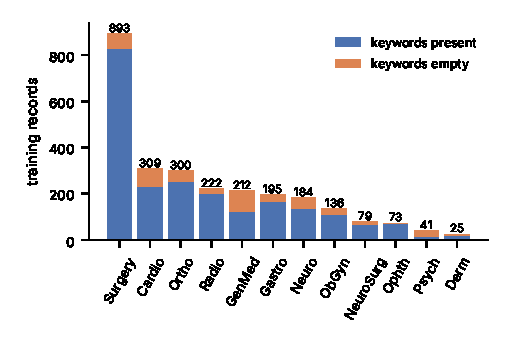
\includegraphics[width=\columnwidth]{figures/class_dist.pdf}
\caption{Training records per specialty, split by whether the keywords field is empty.}
\label{fig:dist}
\end{figure}

\end{document}
